\documentclass[tikz, convert={outfile=backward.svg}]{standalone}
\usepackage{amsmath}
\usepackage{amsbsy}
\usepackage{amsfonts}
\usepackage{amssymb}
\usepackage{amscd}
\usepackage{amsthm}
%\usepackage{mathtools}
\usepackage{graphicx}
\usepackage{tikz}
\usetikzlibrary{calc,fadings,decorations.pathmorphing,decorations.pathreplacing,matrix,arrows,decorations.text,positioning,decorations.markings}
\usepackage{pgfplots}
\tikzset{
    every node/.append style={font=\sffamily}}

\newcommand{\gr}[1]{\textcolor{black!50}{#1}}
\providecommand{\R}{\mathbb{R}}
\begin{document}
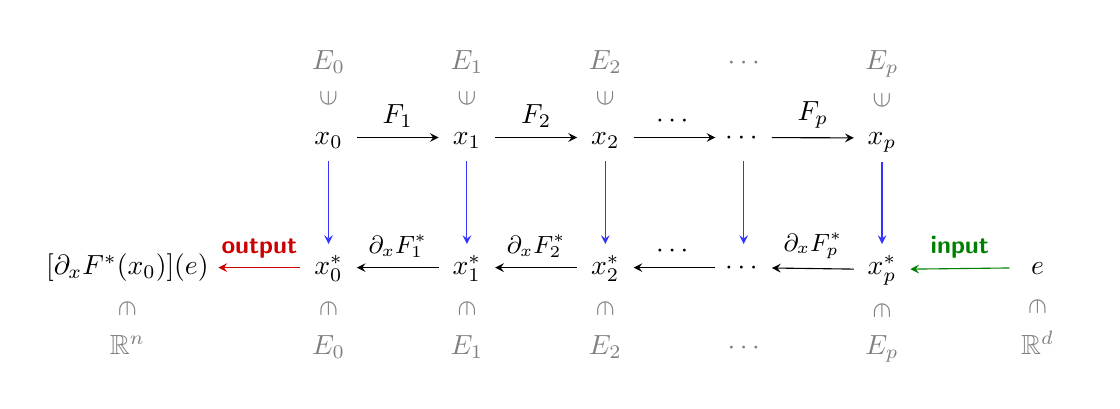
\begin{tikzpicture}%[scale=.4,  every node/.style={scale=0.5} ]
    \matrix (m) [matrix of math nodes,row sep=1em,column sep=3em,minimum width=2em]
    {
        \phantom{\gr{\R^n}} & 
        \gr{{E_0}} & 
        \gr{{E_1}} & 
        \gr{{E_2}} & 
        \gr{\cdots}\vphantom{{E_0}} & 
        \gr{{E_p}} & 
        \phantom{\gr{\R^d}} \\
        \phantom{x_0}\vphantom{F(x_0)_0} & 
        x_0\vphantom{F(x_0)_0} &      
        x_1\vphantom{F(x_0)_0}  &      
        x_2\vphantom{F(x_0)_0}  & 
        \cdots\vphantom{F(x_0)_0}       & 
        x_p\vphantom{F(x_0)_0} & 
        \phantom{F(x_0)}\vphantom{F(x_0)_0}\\[2em]
        {[\partial_x F^*(x_0)] (e)}\vphantom{\partial_x F(x_0)^*} & 
        x_0^*\vphantom{\partial_x F(x_0)^*} &      
        x_1^*\vphantom{\partial_x F(x_0)^*}  &      
        x_2^*\vphantom{\partial_x F(x_0)^*}  & 
        \cdots\vphantom{\partial_x F(x_0)^*}       & 
        x_p^*\vphantom{\partial_x F(x_0)^*} & 
        e\vphantom{\partial_x F(x_0)^*}\\
        \gr{\R^n} & 
        \gr{{E_0}} & 
        \gr{{E_1}} & 
        \gr{{E_2}} & 
        \gr{\cdots}\vphantom{{E_0}} & 
        \gr{{E_p}} & 
    \gr{\R^d}\\};

    \path[-stealth]
    (m-2-2) edge node [above] {$F_1$} (m-2-3)
    (m-2-3) edge node [above] {$F_2$} (m-2-4)
    (m-2-4) edge node [above] {$\cdots$} (m-2-5)
    (m-2-5) edge node [above] {$F_p$} (m-2-6);
    \path[-stealth]
    (m-2-2) edge[color=blue!80!white] (m-3-2)
    (m-2-3) edge[color=blue!80!white] (m-3-3)
    (m-2-4) edge[color=blue!80!white] (m-3-4)
    (m-2-5) edge[color=blue!80!white] (m-3-5)
    (m-2-6) edge[color=blue!80!white] (m-3-6);
    \path[-stealth]
    (m-3-2) edge[color=red!80!black] node [above, color=red!80!black] {\small \textbf{output} } (m-3-1)
    (m-3-3) edge node [above] {\small $\partial_x F_1^*$} (m-3-2)
    (m-3-4) edge node [above] {\small $\partial_x F_2^*$} (m-3-3)
    (m-3-5) edge node [above] {$\cdots$} (m-3-4)
    (m-3-6) edge node [above] {\small $\partial_x F_p^*$} (m-3-5)
    (m-3-7) edge[color=green!50!black] node [above, color=green!50!black] {\small \textbf{input}  } (m-3-6);
    \path
    (m-2-1) -- node[sloped] {} (m-1-1)
    (m-2-2) -- node[sloped] {\gr{$\in$}} (m-1-2)
    (m-2-3) -- node[sloped] {\gr{$\in$}} (m-1-3)
    (m-2-4) -- node[sloped] {\gr{$\in$}} (m-1-4)
    (m-2-6) -- node[sloped] {\gr{$\in$}} (m-1-6)
    (m-2-7) -- node[sloped] {} (m-1-7);
    \path
    (m-3-1) -- node[sloped] {\gr{$\in$}} (m-4-1)
    (m-3-2) -- node[sloped] {\gr{$\in$}} (m-4-2)
    (m-3-3) -- node[sloped] {\gr{$\in$}} (m-4-3)
    (m-3-4) -- node[sloped] {\gr{$\in$}} (m-4-4)
    (m-3-6) -- node[sloped] {\gr{$\in$}} (m-4-6)
    (m-3-7) -- node[sloped] {\gr{$\in$}} (m-4-7);
\end{tikzpicture}

\end{document}
